\documentclass[a4paper]{article}

\usepackage[top=1.2in, bottom=1.2in, left=1in, right=1in]{geometry}
\usepackage{graphicx, minted, textcomp}
\usepackage[T1]{fontenc}

\title{LC2K Hardware Implementation with FPGA}
\author{Rijun Cai\\12348003}

\begin{document}
\maketitle

\section{Introduction}
In this laboratory, I modified the LC2K multiple cycle datapath design in Laboratory 5 and implemented it
in a Diligent\textsuperscript{\textregistered} BASYS 2\texttrademark~board with a
XILINX\textsuperscript{\textregistered} Spartan\texttrademark~3E-100 CP132 FPGA chip.
In addition, I wrote some useful modules and tools to help test my implementation.

\section{Implementation}
\subsection{Adjustments to the Original Design}
Due to the limited resources of the Spartan 3E FPGA chip, some necessary adjustments should be made to
make the design fit in the chip. According to the synthesis report given by the XILINX ISE, the original
overused the slices and IO buffers in the chip. Here is my adjustment scheme.
\begin{enumerate}
    \item Reduce the testing IO ports

        The \verb|LC2K| module had loads of IO ports for testing. Those ports are useless in such an
        implementation. So they were removed except the \verb|outPC|. The saved IOB resources were essential
        for building a more reasonable testing module.

    \item Use Block RAM to implement the main memory

        According to the synthesis report, more than a half of the slices were used to implement the main
        memory (the \verb|TestRAM| module) even if the memory size was reduced to 128Bytes (a bigger memory
        will result in a synthesis failure). In fact, the Spartan-3 generation FPGA chip has four built-in 18Kbits
        (parity bits included) synchronous Block RAM according to the \emph{Spartan-3 Generation FPGA User Guide}.
        So I used the built-in Block RAM to implement the main memory. But the controller in the original design 
        required a asynchronous-read memory, so there are some adjustments in the controller.

    \item Change all registers to synchronous-write

        In the original design, some registers were asynchronous-write, while the others were
        synchronous-write, which would result in difficulities in debugging due to the unpredictable intermediate
        states. So I changed all the registers to synchronous-write.

\end{enumerate}

\subsection{Testing Modules and Tools}
To facilitate debugging, I wanted to display the content of the register file with the 7-segments LEDs on the
BASYS 2 board, so I wrote a module to control the LEDs. The module will control the four 7-segments LEDs to
display a 16 bits digi in hexadecimal form.

To support the display of register file, a process was added to the implementation of the register file.
The process will output the content of the register with a specific address and the lower 16 bits of its output
was connected to the module described above. The address port was connected to the switches so that I can choose
which register to display by the switches.

As mentioned above, the implementation of the main memory was changed to the built-in Block RAM, which has
a different initialization form. So I wrote a python script to automatically convert the machine code file to
the required initialization form. The code is as follow.
\begin{minted}{python}
#!/usr/bin/env python2

if __name__ == '__main__':
    buf = []
    try:
        while True:
            x = input()
            if not (-2 ** 31 <= x < 2 ** 31):
                break
            buf.append(x)
    except (EOFError, TypeError):
        pass

    mem = [['00000000'] * 8 for i in range(0x3F)]
    for addr, ins in enumerate(buf):
        if ins >= 0:
            hex_ins = hex(ins)[2:].upper().rjust(8, '0')
        else:
            hex_ins = hex((1 << 32) + ins)[2:].upper()
        mem[addr >> 3][addr & 0x7] = hex_ins

    for line_addr, line in enumerate(mem):
        print 'INIT_{} => X"{}{}{}{}{}{}{}{}",'.format(
                hex(line_addr)[2:].upper().rjust(2, '0'),
                *reversed(line))
\end{minted}

\subsection{Mapping, Synthesis and Programming}
The \verb|rst| input was mapped to a push button. I would also map the \verb|clk| to a push button sometimes
when debugging so that I could monitor the status in each cycle and I would map it to \verb|MCLK| at last.
The display module required a high frequency clock so I connected it to \verb|MCLK| (through \verb|clk| or
\verb|DISCLK|) all the time. The lower 8 bits of \verb|outPC| was mapped to the LEDs.
The user constraint file is as follow.
\begin{verbatim}
NET "clk" LOC = B8;
#NET "clk" LOC = C11 | CLOCK_DEDICATED_ROUTE = FALSE;
#NET "DISCLK" LOC = B8;
NET "rst" LOC = G12 | CLOCK_DEDICATED_ROUTE = FALSE;

NET "seg<0>" LOC = "L14";
NET "seg<1>" LOC = "H12";
NET "seg<2>" LOC = "N14";
NET "seg<3>" LOC = "N11";
NET "seg<4>" LOC = "P12";
NET "seg<5>" LOC = "L13";
NET "seg<6>" LOC = "M12";

NET "outPC<0>" LOC = "M5";
NET "outPC<1>" LOC = "M11";
NET "outPC<2>" LOC = "P7";
NET "outPC<3>" LOC = "P6";
NET "outPC<4>" LOC = "N5";
NET "outPC<5>" LOC = "N4";
NET "outPC<6>" LOC = "P4";
NET "outPC<7>" LOC = "G1";

NET "an<0>" LOC = "K14";
NET "an<1>" LOC = "M13";
NET "an<2>" LOC = "J12";
NET "an<3>" LOC = "F12";

NET "Test_address<2>" LOC = "K3";
NET "Test_address<1>" LOC = "L3";
NET "Test_address<0>" LOC = "P11";
\end{verbatim}

Then I used XILINX ISE to synthesize the design. According to the synthesis report, the highest clock
frequency of my design is about 69MHz. So I chose 50MHz for \verb|MCLK|. Then I used XILINX iMPACK to
generate the PROM file and program it to the board.

\section{Tests and Results}
I tested the implementation with some LC2K programs and compared the final states of the register file
with those from the XILINX iSim simulator and the simulator finished in Laboratory 2. And they three
gave identical results. One of the tests are described as follow.

The test program calculates the 20th term of the Fibonacci sequence with a tail-call optimized recursive
algorithm. The code is as follow.
\begin{minted}{gas}
init        lw      0   7   sp
            lw      0   1   n
            lw      0   5   const+2
            lw      0   3   const+1     fib(R5)
            lw      0   2   const+1     fib(R5 - 1)
            lw      0   4   fib-addr
            jalr    4   6
            halt
fib         beq     1   5   end
            lw      0   4   const-1
            add     7   4   7
            sw      7   6   1
            add     0   3   4
            add     3   2   3
            add     0   4   2
            lw      0   4   const+1
            add     5   4   5
            lw      7   6   1
            add     7   4   7
            beq     0   0   fib
end         jalr    6   4
sp          .fill   255
fib-addr    .fill   fib
const-1     .fill   -1
const+1     .fill   1
const+2     .fill   2
n           .fill   20
\end{minted}
\newpage
The final state of the register file in \verb|simulate| is:
\begin{verbatim}
reg[ 0 ] 0
reg[ 1 ] 20
reg[ 2 ] 4181
reg[ 3 ] 6765
reg[ 4 ] 21
reg[ 5 ] 20
reg[ 6 ] 7
reg[ 7 ] 255
\end{verbatim}

The final state of the register file in XILINX iSim is shown in Figure~\ref{fig:isim}.
\begin{figure}[ht!]
    \center
    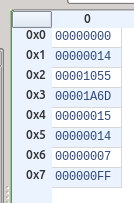
\includegraphics[scale=0.6]{isim}
    \caption{Final State of the Register File in iSim}\label{fig:isim}
\end{figure}

The final state of the register file in the FPGA is shown in Figure~\ref{tab:fpga}.

\begin{figure}[ht!]
    \center
    \begin{tabular}{c|c}
        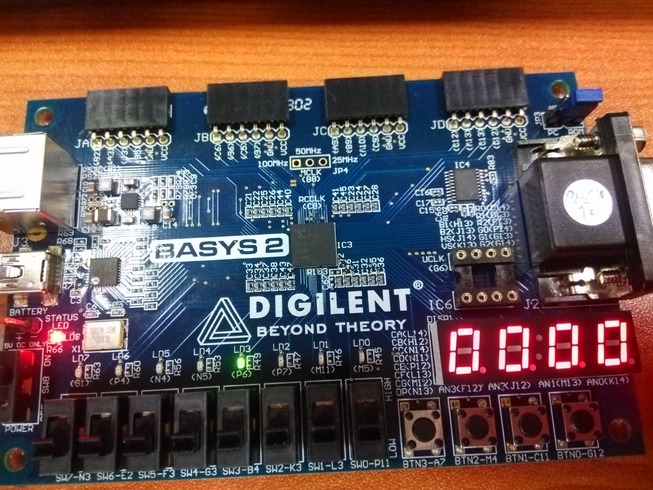
\includegraphics[scale=0.3]{reg0}&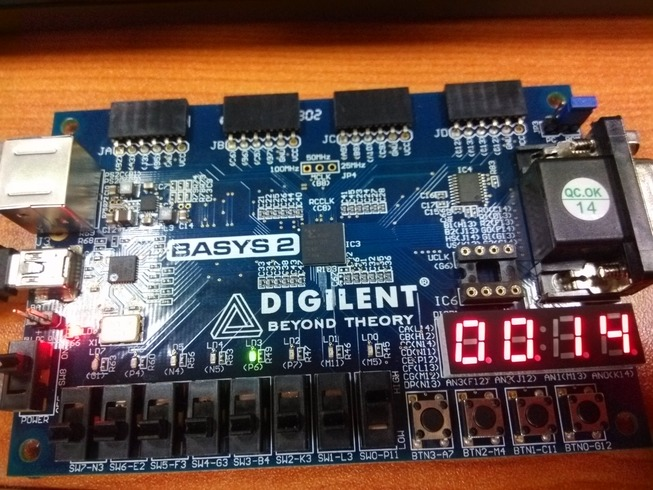
\includegraphics[scale=0.3]{reg1}\\
        Final State of the Reg0\label{fig:reg0}&Final State of the Reg1\label{fig:reg1}
        \\
        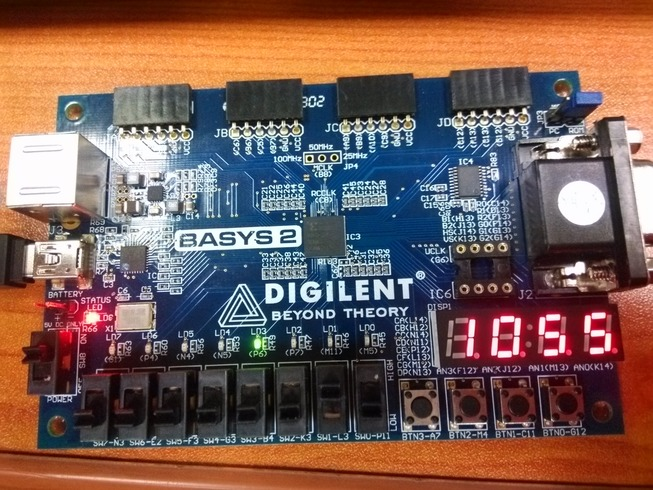
\includegraphics[scale=0.3]{reg2}&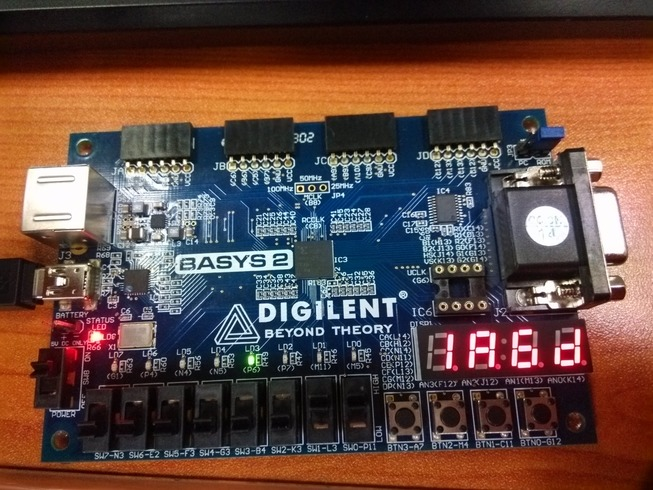
\includegraphics[scale=0.3]{reg3}\\
        Final State of the Reg2\label{fig:reg2}&Final State of the Reg3\label{fig:reg3}
        \\
        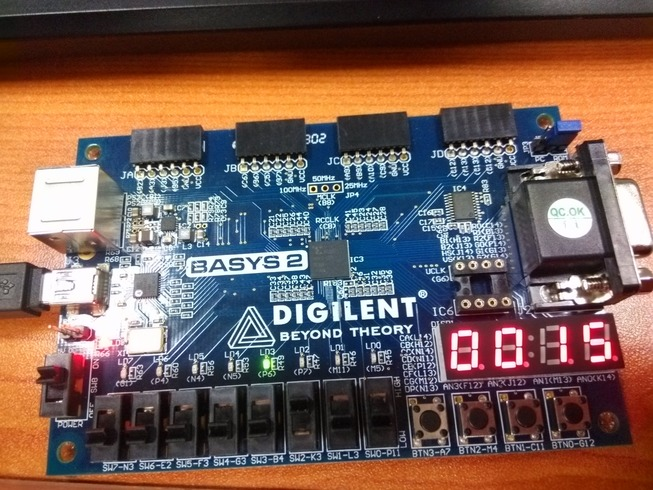
\includegraphics[scale=0.3]{reg4}&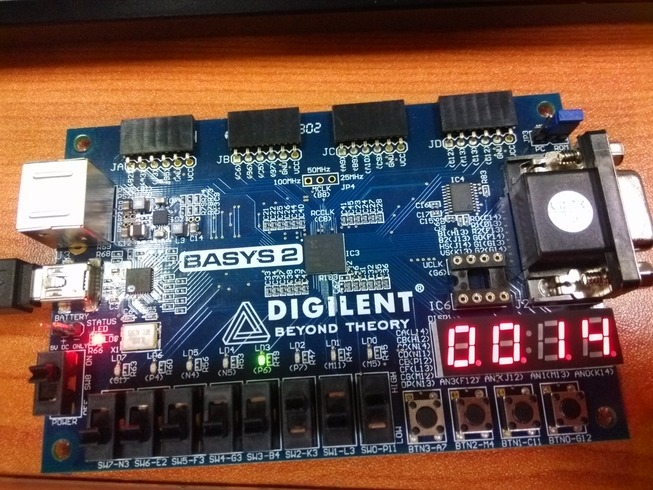
\includegraphics[scale=0.3]{reg5}\\
        Final State of the Reg4\label{fig:reg4}&Final State of the Reg5\label{fig:reg5}
        \\
        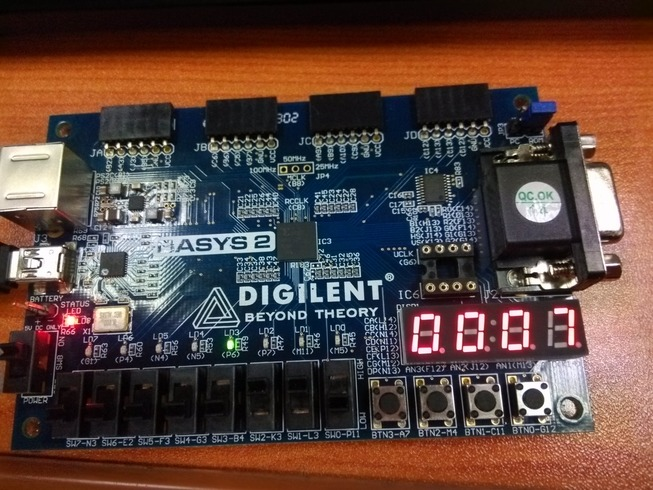
\includegraphics[scale=0.3]{reg6}&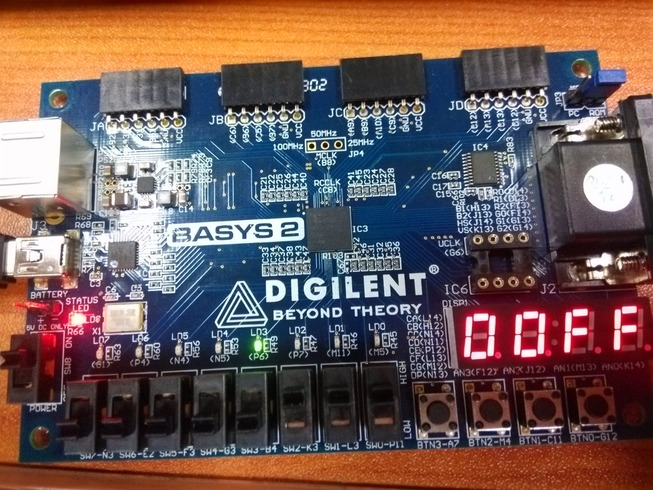
\includegraphics[scale=0.3]{reg7}\\
        Final State of the Reg6\label{fig:reg6}&Final State of the Reg7\label{fig:reg7}
    \end{tabular}
    \caption{Final State of the Register File in the FPGA}\label{tab:fpga}
\end{figure}

\end{document}
